\documentclass[
	12pt,
	a4paper,
	bibtotoc,
	cleardoubleempty, 
	idxtotoc,
	%ngerman,
	english,
	%openright,
	%final,
	openany,	% lässt neue Kapitel auch auf geraden Seiten beginnen
	listof=nochaptergap,
	]{scrbook}

\usepackage{cmap}
\usepackage[T1]{fontenc}
\usepackage[utf8]{inputenc}

% ##################################################
% Document variables
% ##################################################

% Personal data of the autor
\newcommand{\docSurname}{Schmutz}
\newcommand{\docPrename}{Yannis}
\newcommand{\docStreet}{Hildanusstrasse 18}
\newcommand{\docLocation}{Bern}
\newcommand{\docZip}{3013}
\newcommand{\docEmail}{yannisvalentin.schmutz@students.bfh.ch}
\newcommand{\docStudentnumber}{17-253-949}


% Data of the University
\newcommand{\docLocationFH}{Bern}
\newcommand{\docFieldOfStudy}{BSc Computer Science}


% Document data
\newcommand{\docTitle}{SleepO}
%\newcommand{\docSecondTitle}{} % No second title
\newcommand{\docSecondTitle}{Time Series Clustering Approach}
\newcommand{\docKindOfWork}{Project documentation clustering of time series data}
\newcommand{\docHandOverDate}{TBD}
\newcommand{\docFirstLector}{Vidushi Christina Bigler}
%\newcommand{\docSecondLector}{-} % If there is only one lector
\newcommand{\docSecondLector}{-}

% Used for toggle-if case
\usepackage{etoolbox}

% Conditional variables
\providetoggle{useCode}
\settoggle{useCode}{true}
\providetoggle{useAbstract}
\settoggle{useAbstract}{true}

% ##################################################
% General packages
% ##################################################

% Set language to english
%\usepackage[english,spanish,swedish,portuges,german]{babel}
\usepackage[english]{babel}


% Use graphics
\usepackage{graphicx}

% Additional special characters
\usepackage{dingbat}


% Colors
\usepackage{color}
\usepackage[usenames,dvipsnames,svgnames,table]{xcolor}

% Masking of URLs and file paths
\usepackage[hyphens]{url}

% German quotes
%\usepackage[babel, german=quotes]{csquotes}

% Package for indexing (Schlagwortverzeichnis)
\usepackage{index}
\makeindex

% Ipsum Lorem
\usepackage{lipsum}


% ##################################################
% Page formatting
% ##################################################
\usepackage[
	portrait,
	%bindingoffset=1.5cm,	% Aktivieren, wenn das Dokument gebunden werden soll
	inner=2.5cm, % Left margin
	outer=2.5cm, % Right marin
	top=1.5cm,   
	bottom=2cm,   
	includefoot,
	includehead
	%showframe,  % Aktivieren um Seitengrenzen anzuzeigen
	%includeheadfoot
	]{geometry}

% ##################################################
% Header and footer
% ##################################################

\usepackage{fancyhdr}

\pagestyle{fancy}
\fancyhf{}
\fancyhead[EL,OR]{\sffamily\thepage}
\fancyhead[ER,OL]{\sffamily\nouppercase{\leftmark}}

\fancyfoot[LE,LO]{Bern University of Applied Sciences}
\fancyfoot[RE,RO]{\docPrename~\docSurname}
% For two authors use:
% \fancyfoot[RE,RO]{\docPrename~\docSurname, \docPrenameB~\docSurnameB}
\renewcommand{\footrulewidth}{1pt}		% add footer line by setting it to one


\fancypagestyle{headings}{}

\fancypagestyle{plain}{}

% No header/footer on empty pages
\fancypagestyle{empty}{
  \fancyhf{}
  \renewcommand{\headrulewidth}{0pt}
  \renewcommand{\footrulewidth}{0pt}
}


%Saves \chaptermark in \oldchaptermark so that 
% it can be reset for the appendix
\let\oldchaptermark\chaptermark

%No "Chapter # NAME" in header
\renewcommand{\chaptermark}[1]{
	\markboth{#1}{}
   	\markboth{\thechapter.\ #1}{}
}

% ##################################################
% fonts
% ##################################################

% Set default font
\renewcommand{\familydefault}{\sfdefault}

% Set default line distance to 1.5
\usepackage{setspace}
\onehalfspacing 

% Set font size
\addtokomafont{chapter}{\sffamily\Large\bfseries} 
\addtokomafont{section}{\sffamily\large\bfseries} 
\addtokomafont{subsection}{\sffamily\normalsize\bfseries} 
\addtokomafont{caption}{\sffamily\normalsize\mdseries} 

%Disable indent of paragraphs
\setlength{\parindent}{0pt}

%Line distances of paragraphs
\usepackage{parskip}

% ##################################################
% Table of contents / General listings
% ##################################################

\usepackage{tocloft}

% Points also for chapters
\renewcommand{\cftchapdotsep}{3}
\renewcommand{\cftdotsep}{3}

% Adjust font and size in table of contents
\renewcommand{\cftchapfont}{\sffamily\normalsize}
\renewcommand{\cftsecfont}{\sffamily\normalsize}
\renewcommand{\cftsubsecfont}{\sffamily\normalsize}
\renewcommand{\cftchappagefont}{\sffamily\normalsize}
\renewcommand{\cftsecpagefont}{\sffamily\normalsize}
\renewcommand{\cftsubsecpagefont}{\sffamily\normalsize}

%Set space between lines in listings
\setlength{\cftparskip}{.5\baselineskip}
\setlength{\cftbeforechapskip}{.1\baselineskip}


% ##################################################
% Table of figures and figures
% ##################################################

\usepackage{caption}

\usepackage{wrapfig}

% Numbering of figures
\renewcommand{\thefigure}{\arabic{figure}}
\usepackage{chngcntr}
\counterwithout{figure}{chapter}

% Adjust table of figures
\renewcommand{\cftfigpresnum}{Figure }
\renewcommand{\cftfigaftersnum}{:}

% Width of numbering scope [Figure 1:]
\newlength{\figureLength}
\settowidth{\figureLength}{\bfseries\cftfigpresnum\cftfigaftersnum}
\addtolength{\figureLength}{2mm} %extra offset
\setlength{\cftfignumwidth}{\figureLength}
\setlength{\cftfigindent}{0cm}

% Adjust font
\renewcommand\cftfigfont{\sffamily}
\renewcommand\cftfigpagefont{\sffamily}

%Default paths
\graphicspath{ {./content/pictures/} {../../src/images/reference/} {../../src/images/clustering/} }

% ##################################################
% List of tables and tables
% ##################################################

% Numbering of tables
\renewcommand{\thetable}{\arabic{table}}
\counterwithout{table}{chapter}

% Adjust list of tables
\renewcommand{\cfttabpresnum}{Table }
\renewcommand{\cfttabaftersnum}{:}

% Width of numbering scope [Table 1:]
\newlength{\tableLength}
\settowidth{\tableLength}{\bfseries\cfttabpresnum\cfttabaftersnum}
\addtolength{\tableLength}{3mm} %extra offset
\setlength{\cfttabnumwidth}{\tableLength}
\setlength{\cfttabindent}{0cm}

%Adjust font
\renewcommand\cfttabfont{\sffamily}
\renewcommand\cfttabpagefont{\sffamily}

% Suppress vertical lines
\usepackage{booktabs}

%Multi row for specific rows
\usepackage{multirow}

%Additional table package
\usepackage{tabu}


% ##################################################
% Listings (Sourcecode)
% ##################################################

\usepackage{listings}

%use typewriter font which supports bold characters
\usepackage{beramono}

\definecolor{codegreen}{rgb}{0,0.6,0}
\definecolor{codegray}{rgb}{0.5,0.5,0.5}
\definecolor{codepurple}{rgb}{0.5,0,0.33}
\definecolor{codepurblue}{rgb}{0.16,0.0,1.0}
\definecolor{backcolour}{rgb}{0.95,0.95,0.92}


% TODO: Set Python colors
\lstdefinestyle{codestyle}{
    backgroundcolor=\color{backcolour},   
    commentstyle=\color{codegreen},
    keywordstyle=\bfseries\color{codepurple},
    numberstyle=\tiny\color{codegray},
    stringstyle=\color{codepurblue},
    basicstyle=\scriptsize\ttfamily,
    breakatwhitespace=false,         
    breaklines=true,                 
    captionpos=b,                    
    keepspaces=true,                 
    numbers=left,                     
    numbersep=5pt,                 
    showspaces=false,                
    showstringspaces=false,
    showtabs=false,                  
    tabsize=2
}

\lstset{style=codestyle}

%Import code snippet from file
%\mylisting{from}{to}{language}{file}{descr}{path}
\newcommand{\mylisting}[6]{
\lstinputlisting[language=#3,
				firstnumber=#1,
				firstline=#1,
				lastline=#2,
				caption={#4, #5}, 
				label={implementation_listing_#4_#5}]
				{#6}
}

% ##################################################
% Appendix
% ##################################################

%Calc packet for calculations
\usepackage{calc}
\usepackage{amsmath}

%Appendix packet, set the flags for the TOC
\usepackage[toc,title,titletoc]{appendix} 


% Change text for title
%\renewcommand{\appendixtocname}{Appendix}

%Befehl für einen neuen Bericht und die erste Seite als Bild
\newcommand{\appendixsection}[2]{
\section{#1}
\appendixsingle{#2}
}

%Befehl für einzelne Seite als Bild eingefasst, damit Überschrift und Kopfzeile
% bestehen bleibt. 
\newcommand{\appendixsingle}[1]{
\vspace{-10cm}
\vfill
\mbox{}\hspace{-1.5cm}\includegraphics[width=\linewidth+3cm]{#1}\hspace{-1.5cm}\mbox{}
\vspace{-10cm}
\vfill
\mbox{}
}

%Datenträger Tabelle
\definecolor{lightgray}{gray}{0.85}
\definecolor{ultralightgray}{gray}{0.95}
\definecolor{mygray}{gray}{0.70}

% ##################################################
% Theoreme
% ##################################################

% TODO: English?
% Umgebung fuer Beispiele
\newtheorem{beispiel}{Beispiel}

% TODO: English?
% Umgebung fuer These
\newtheorem{these}{These}

% Umgebung fuer Definitionen
\newtheorem{definition}{Definition}
  	
% ##################################################
% Literaturverzeichnis
% ##################################################

\usepackage{bibgerm}

% ##################################################
% Abkuerzungsverzeichnis
% ##################################################

%\usepackage[printonlyused]{acronym}
\usepackage{acronym}

% ##################################################
% PDF / Dokumenteninternelinks
% ##################################################

\usepackage[
	colorlinks=false,
   	linkcolor=black,
   	citecolor=black,
  	filecolor=black,
	urlcolor=black,
    bookmarks=true,
    bookmarksopen=true,
    bookmarksopenlevel=3,
    bookmarksnumbered,
    plainpages=false,
    pdfpagelabels=true,
    hyperfootnotes,
    hidelinks,
    pdftitle ={\docTitle},
    pdfauthor={\docPrename~\docSurname},
    pdfcreator={\docPrename~\docSurname}]{hyperref}

% ####################################################
% Command für einfache Quellenangabe bei Bilder, etc.
% ####################################################

% TODO: English?
\newcommand{\source}[1]{\caption*{Quelle: {#1}} }



% ####################################################
% Dynamisches Feature-handling
% ####################################################

% TODO
% Aus CSV Files Tabellen erstellen können
\usepackage{csvsimple}
\newcommand{\myCsvDataPath}{../../src/data/}
\newcommand{\myRawCsvDataPath}{\myCsvDataPath/raw/}
\newcommand{\myCleanedCsvDataPath}{\myCsvDataPath/cleaned/}


%\newcommand{\myFeaturePath}{../../src/data_visualization/}
%\newcommand{\myDataOverviewPath}{\myFeaturePath/data_overview/}
%\newcommand{\myFeatureDescriptionPath}{\myFeaturePath/feature_descriptions/}

% Be able to use multiple columns in itemize
\usepackage{multicol}




% Beginn des Dokuments
\begin{document}

\setcounter{secnumdepth}{3}

% Titelblatt
\begin{titlepage}
\pagestyle{empty}

% ##################################################
% BFH-Logo einbinden
% ##################################################
\begin{flushleft}
\begin{figure}[ht]
\flushleft

\includegraphics[height=3cm]{content/pictures/bfh_logo.jpeg}
\end{figure}
\end{flushleft}

% ##################################################
% Titel
% ##################################################
\begin{center}
{\fontsize{18}{22} \selectfont \docKindOfWork}\\[5mm]
{\fontsize{18}{22} \selectfont in the course of study} \\[5mm]
{\fontsize{18}{22} \selectfont \docFieldOfStudy}\\
\vspace{1cm}

\begin{onehalfspace}
% TODO: SleepO-Logo?
%\begin{figure}[h!]
%		\centering
%		\includegraphics[width=0.4\textwidth]{logo.jpg}
%		\label{fig:titelbild}
%\end{figure}
{\fontsize{18}{22} \selectfont \docSecondTitle}


\end{onehalfspace}
\end{center}

% ##################################################
% Zusatzinformationen
% ##################################################
\vfill
\begin{center}
\begin{tabular}{lcl}
Lector  		&:& \docFirstLector 	\\ \\
%Koreferent 		&:& \docSecondLector \\ \\
Submitted at	&:& \docHandOverDate 	\\ \\
Submitted by 	&:& \docPrename~\docSurname\\
				& & Matriculation number: \docStudentnumber\\
				& & \docStreet,~\docZip~\docLocation\\
				& & \docEmail
					
\end{tabular}
\end{center}
\end{titlepage}
\cleardoubleemptypage

\frontmatter
\pagenumbering{Roman}

\iftoggle{useAbstract}{
	% Abstract
	\chapter*{Abstract\markboth{Abstract}{}}
\addcontentsline{toc}{chapter}{Abstract}

Foooo Baaar
	%\cleardoubleemptypage
	\clearpage
}

% Inhaltsverzeichnis
\phantomsection
\addcontentsline{toc}{chapter}{Contents}
\tableofcontents
\cleardoubleemptypage

% Abbildungsverzeichnis einbinden und ins Inhaltsverzeichnis
% WORKAROUND: tocloft und KOMA funktionieren zusammen nicht
% korrekt\phantomsection
\phantomsection 
\addcontentsline{toc}{chapter}{\listfigurename} 
\listoffigures
%\cleardoubleemptypage
\clearpage

% Tabellenverzeichnis einbinden und ins Inhaltsverzeichnis
% WORKAROUND: tocloft und KOMA funktionieren zusammen nicht
% korrekt\phantomsection
\phantomsection
\addcontentsline{toc}{chapter}{\listtablename}
\listoftables
%\cleardoubleemptypage
\clearpage

% Quellcodeverzeichnis nur anzeigen, wenn useCode auf true ist
\iftoggle{useCode}{

% TODO: Fix this or build it myself

% Quellcodeverzeichnis einbinden und ins Inhaltsverzeichnis
%\phantomsection
%\addcontentsline{toc}{chapter}{Quellcodeverzeichnis}

%Define listing
%\makeatletter
%\begingroup
%  \let\newcounter\@gobble\let\setcounter\@gobbletwo
%  \globaldefs\@ne \let\c@loldepth\@ne
%  \newlistof{listings}{lol}{\lstlistlistingname}
%\endgroup
%\let\l@lstlisting\l@listings
%\makeatother
%\setlength{\cftlistingsindent}{0em}
%\renewcommand{\cftlistingsafterpnum}{\vskip0pt} %Spacing between entries
%\renewcommand*{\cftlistingspresnum}{\lstlistingname~}
%\settowidth{\cftlistingsnumwidth}{\cftlistingspresnum}
%\renewcommand{\lstlistlistingname}{Quellcodeverzeichnis}
%% Tabellenverzeichnis anpassen
%\renewcommand{\lstlistingname}{Codeauschnitt}
%\renewcommand{\cftlistingsaftersnum}{:}
%% Breite des Nummerierungsbereiches [Codeauschnitt 1:]
%\newlength{\codeLength}
%\settowidth{\codeLength}{\bfseries\lstlistingname\cftlistingsaftersnum}
%\addtolength{\codeLength}{5mm}
%\setlength{\cftlistingsnumwidth}{\codeLength}
%\lstlistoflistings
%\cleardoubleemptypage
}

% Abkürzungsverzeichnis
\chapter*{List of Abbreviations \markboth{List of Abbreviations}{}}
\addcontentsline{toc}{chapter}{List of Abbreviations}

\begin{acronym}
	\acro{b2b}[B2B]{Beat-to-Beat Time}
	\acro{bfh}[BFH]{Bern University of Applied Sciences}
	\acro{csv}[CSV]{Comma Separated Value}
	\acro{cvi}[CVI]{Cluster Validity Indice}	
	\acro{dtw}[DTW]{Dynamic Time Warping}
	\acro{hr}[HR]{Heart Rate}
	\acro{mss}[MSS]{Measured Signal Strength}
	\acro{rem}[REM]{Rapid Eye Movement}
	\acro{rr}[RR]{Respiration Rate}
	\acro{ss}[SS]{Signal Strength}
\end{acronym}

\mainmatter

% Include chapters here:
\chapter{Introduction}

BlaaaaBlaaa

\section{Initial position}

BlaaaaBlaaa


\section{Project goal}

BlaaaaBlaaa

\section{Requirements}

Bluuuu

\chapter{Approach}

Blablabsdjkfb

\section{Reference time series data ser}

\chapter{Data}

This chapter describes the background of the data, how it is produced and the expected format.

\section{Source}
The data comes form several medical sensors which are mounted to the bed of the corresponding proband. The sensors send their data in configured intervals to a data pipeline. The pipeline then transforms the data and then saves it in a Postgres DB.

\section{Format}
\label{c:data_format}

The source of the data for this project is stored in a database which implements a star-schema. The data is daily exported to CSV files for each proband using trivial join expressions.

All time series are recorded from 8:00 PM to 10:00 AM.
The sampling granularity is one second. However due to the sensors behaviour, some data points are missing every 30s.
Due to the fine granularity this is negligible.

If data would be sent every second without missing data, each time series would be $14\cdot3600 = 50400$ rows long. However the length is usually around 48000.

\clearpage
The given CSV then contains the following columns:

\begin{multicols}{2}
\begin{itemize}
  \item id
  \item heart\_rate
  \item respiration\_rate
  \item relative\_stroke\_volume
  \item heart\_rate\_variability
  \item measured\_signal\_strength
  \item status
  \item b2b1
  \item b2b2
  \item b2b3
  \item date
  \item day
  \item month
  \item year
  \item location\_name
  \item room
  \item patient
  \item sensor
  \item hour
  \item minute
  \item second
\end{itemize}
\end{multicols}

During the preparation and cleaning process the attributes "date", "hour", "minute" and "second" are used in order to create the timestamps.
For now, the focus will lie on the features "heart\_rate" and "respiration\_rate".


\section{Cleaning}
Due to the fact that real world data is used, some work has to to be put into data cleaning. This work is done in the Jupyter Notebook "CleanAllRawData.ipynb". It is well documented so have a look at it for more information.


The sensor sometimes is not able to detect a signal although the person is in bed. In such case it will send 0-values. Therefore the values of e.g \ac{hr} and \ac{rr} jump quite often to zero.

However even if no heart rate or respiration rate can be detected, the \ac{mss} will produce a high value. Observations have shown, that if the \ac{mss} is below a given threshold (e.g 715) the bed is actually not occupied. In this case the zero-values sent by the sensor are legit. If the \ac{mss} is above the threshold but \ac{hr} and \ac{rr} are zero, this must be considered as missing value.

The forward fill will produce a slight look ahead bias. But due to the fine granularity of the data and the downsampling to come, this is negligible.

We replace these values using a custom forward fill. Figure \ref{fig:forward_fill_example} displays the original time series of \ac{hr} (blue) and the resulting time series after the forward fill algorithm.

\begin{figure}[h!]
	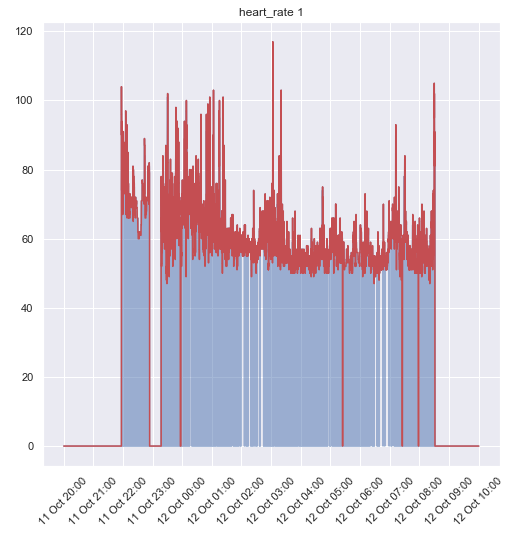
\includegraphics[width=1.1\textwidth]{/forward_fill_example.png}
	\caption{Example of the forward fill output}
	\label{fig:forward_fill_example}
\end{figure}


\newpage
Running time series clustering algorithms is very expensive (regarding computation costs). Therefore the datasets have to been downsampled to different granularities. At the moment the granularities 

\begin{itemize}
	\item 1 hour
	\item 30 minutes
	\item 5 minutes
	\item 1 minute
\end{itemize}

are provided.



\section{Used time series}
After cleaning the raw time series it will be available with the rows \textbf{timestamp}, \textbf{heart rate}, \textbf{respiration rate}, \textbf{mss} and \textbf{patient}. As shown in table \ref{tab:example_ts_one_h_granularity}.


\begin{table}[h!]
\centering
\resizebox{\textwidth}{!}{
	\begin{tabular}{|c|c|c|c|c|}\hline%
		% specify table head
		\bfseries timestamp & 
		\bfseries heart\_rate &
		\bfseries respiration\_rate &
		\bfseries mss &
		\bfseries patient
		
		\csvreader[]{\myCleanedCsvDataPath/samples50/one_hour/yyyyy_1.csv}{
			1=\myTS,2=\myHR,3=\myRR,
			4=\myMSS,5=\myPAT} % specify your columns here
			{\\\hline\myTS & \myHR & \myRR & 
			\myMSS & \myPAT}
		\\\hline	
	\end{tabular}
}
\caption{Example One hour granularity data}
\label{tab:example_ts_one_h_granularity}
\end{table}

For every granularity there are 50 different time series stored in \path{src/data/cleaned/samples/}. Four of them had been synthetically generated using the jupyter notebook \path{synth_data_generator.ipynb}. This was necessary because four data sets had to be discarded during the data cleaning process.

\chapter{Reference Data}

Blablabsdjkfb


\section{Foo}



\begin{table}[h!]
\centering
\resizebox{\textwidth}{!}{
	\begin{tabular}{|c|c|c|c|c|}\hline%
		% specify table head
		\bfseries timestamp & 
		\bfseries heart\_rate\_1 &
		\bfseries respiration\_rate\_1 &
		\bfseries heart\_rate\_2 &
		\bfseries respiration\_rate\_2
		
		\csvreader[]{\myCleanedCsvDataPath/reference/ref_1hour.csv}{
			1=\myTS,2=\myHRa,3=\myRRa,
			4=\myHRb,5=\myRRb} % specify your columns here
			{\\\hline\myTS & \myHRa & \myRRa & 
			\myHRb & \myRRb}
		\\\hline	
	\end{tabular}
}
\caption{Reference timeseries 1 hour}
\label{tab:ref_ts_1h}
\end{table}


\chapter{Reference Distance}

This chapter describes the result of the distance measurements for the defined reference data. All calculations and graphs shown in this chapter are produced in the Jupyter Notebook 
\newline \path{DistanceReferenceMeasurement.ipynb}.

\section{One Hour Reference Time Series}

Due to the rough granularity of one hour both distance measures produce the same result. This is also visualised by the straight diagonal red line in figure \ref{fig:ref_dtw_dist_one_h_granularity}.

\subsection{Euclidean Distance}

The Euclidean Distance between the \ac{hr} time series is: \textbf{0.198673}


The Euclidean Distance between the \ac{rr} time series is: \textbf{0.316962}


\subsection{DTW}

The distance using \ac{dtw} between the \acp{hr} values is: \textbf{0.198673}


The distance using \ac{dtw} between the \acp{rr} values is: \textbf{0.316962}

\begin{figure}[h!]
	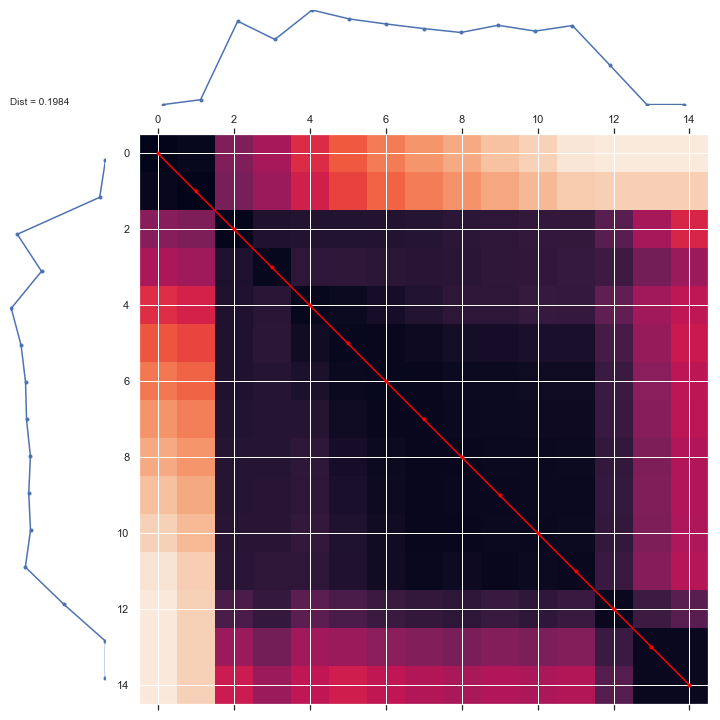
\includegraphics[width=1\textwidth]{ref_1hour_hr_dtw.png}
	\caption{DTW visualisation (HR, 1h granularity)}
	\label{fig:ref_dtw_dist_one_h_granularity}
\end{figure}




\clearpage
\section{30 Minutes Reference Time Series}

Due to the rough granularity of 30min there is no big difference between the Euclidean and \ac{dtw} method. As one can see in figure \ref{fig:ref_dtw_dist_30_min_granularity}, the warping path is still almost a straight diagonal line.

\subsection{Euclidean Distance}

The Euclidean Distance between the \ac{hr} time series is: \textbf{0.369976}


The Euclidean Distance between the \ac{rr} time series is: \textbf{0.775827}


\subsection{DTW}

The distance using \ac{dtw} between the \acp{hr} values is: \textbf{0.327602}


The distance using \ac{dtw} between the \acp{rr} values is: \textbf{0.775718}

\begin{figure}[h!]
	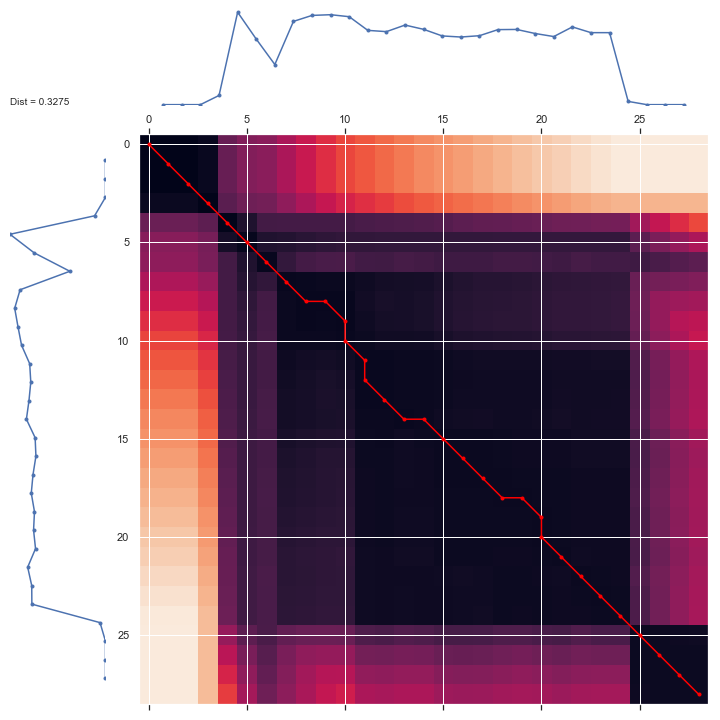
\includegraphics[width=0.7\textwidth]{ref_30min_hr_dtw.png}
	\caption{DTW visualisation (HR, 30min granularity)}
	\label{fig:ref_dtw_dist_30_min_granularity}
\end{figure}


\clearpage
\section{Five Minutes Reference Time Series}

Due to the finer granularity there will bigger differences between the two time series in terms of noise. Thus, the Euclidean and \ac{dtw} distances increase. Therefore, \ac{dtw} have a greater impact than in the previous observations as figure \ref{fig:ref_dtw_dist_5_min_granularity} indicates.

\subsection{Euclidean Distance}

The Euclidean Distance between the \ac{hr} time series is: \textbf{2.095002}


The Euclidean Distance between the \ac{rr} time series is: \textbf{3.644268}


\subsection{DTW}

The distance using \ac{dtw} between the \acp{hr} values is: \textbf{1.600346}


The distance using \ac{dtw} between the \acp{rr} values is: \textbf{2.585769}

\begin{figure}[h!]
	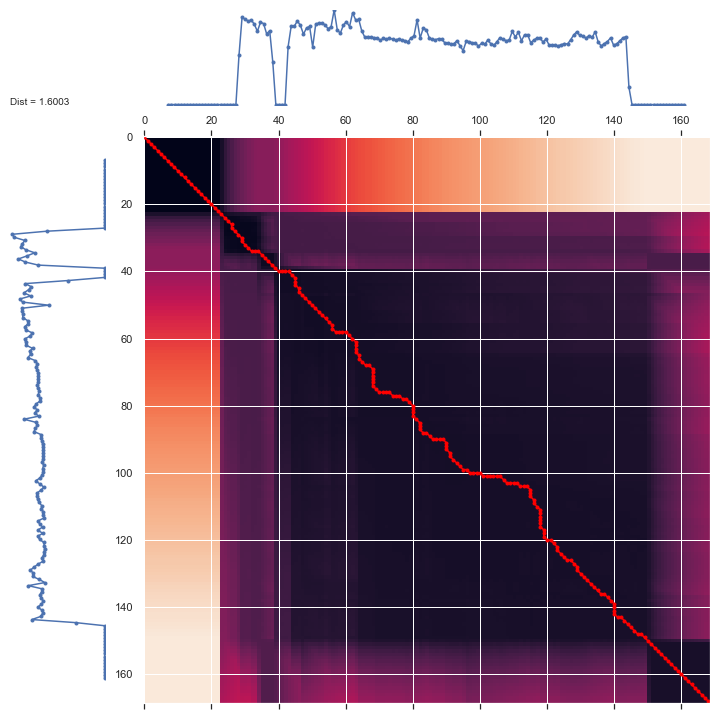
\includegraphics[width=0.7\textwidth]{ref_5min_hr_dtw.png}
	\caption{DTW visualisation (HR, 5min granularity)}
	\label{fig:ref_dtw_dist_5_min_granularity}
\end{figure}






\clearpage
\section{One Minute Reference Time Series}

Now, for the granularity of one minute the \ac{dtw} distance is almost only half of the euclidean distance.

\subsection{Euclidean Distance}

The Euclidean Distance between the \ac{hr} time series is: \textbf{7.455447}


The Euclidean Distance between the \ac{rr} time series is: \textbf{10.56793}


\subsection{DTW}

The distance using \ac{dtw} between the \acp{hr} values is: \textbf{3.888863}


The distance using \ac{dtw} between the \acp{rr} values is: \textbf{5.810633}

\begin{figure}[h!]
	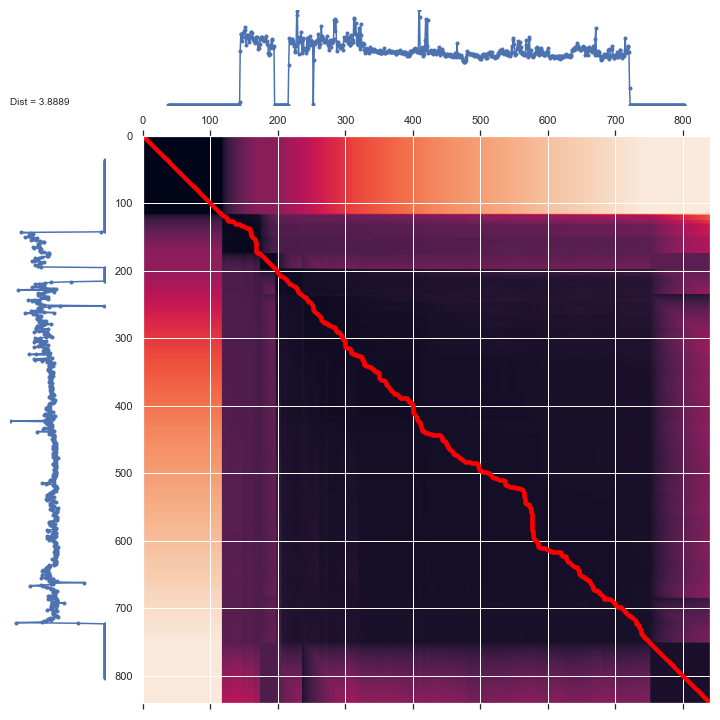
\includegraphics[width=0.7\textwidth]{ref_1min_hr_dtw.png}
	\caption{DTW visualisation (HR, 1min granularity)}
	\label{fig:ref_dtw_dist_1_min_granularity}
\end{figure}


\clearpage
\section{Conclusion}

Table \ref{tab:ref_dist_compare} provides an overview over the calculated reference distances. One can clearly see that the finer the granularity gets the larger the distances will become. Similarly the ratios of the euclidean distance and the \ac{dtw} distance increase.

\begin{table}[h!]
\centering
\resizebox{\textwidth}{!}{
	\begin{tabular}{|c|c|c|c|c|}\hline
		{} &  
		\multicolumn{2}{|c|}{\textbf{\ac{hr}}} & 
		\multicolumn{2}{|c|}{\textbf{\ac{rr}}}\\
		\hline
		% specify table head
		\bfseries Granularity & 
		\bfseries Euclidean &
		\bfseries \ac{dtw} &
		\bfseries Euclidean &
		\bfseries \ac{dtw} \\
		\hline\hline
		1 Hour & 0.198673 & 0.198673 & 0.316962 & 0.316962 \\
		\hline
		30 Min & 0.369976 & 0.327602 & 0.775827 & 0.775718 \\
		\hline
		5 Min & 2.095002 & 1.600346 & 3.644268 & 2.585769 \\
		\hline
		1 Min & 7.455447 & 3.888863 & 10.56793 & 5.810633 \\
		\hline

	\end{tabular}
}
\caption{Reference Distances Comperation}
\label{tab:ref_dist_compare}
\end{table}

Whenever a distance between two time series will be calculated during this project, it can be compared to these reference distances in order to determine "how good/bad" the distance actually is.








\chapter{Conclusion}

\section{Summary}

The main goal of this project, getting familiar with time series clustering, was clearly reached. I learned the fundamental approach on how to tacke a time series clustering problem. I got to know various distance measures, clusterings algorithms and CVI and learned how to practically apply them.

The clustering on the used sleeping data was indeed not groundbreaking but I was able to group some time series together depending on different patterns of the data.


\section{Outlook}

In order to get more out of time series clustering possibilities the following tasks may be tried out in the future:


\begin{itemize}
  \item Use other algorithms than k-Means
  \item Use other data points than "heart rate". E.g:
  \begin{itemize}
  	\item Respiration rate
  	\item Signal strength
  \end{itemize}
  \item Go for a multivariate approach
  \item Use the same kind of bed and mounting position of the sensor for every proband
  \item Cluster the data using subsequence time series clustering
  \item Gather and use even more data
  \item Verify whether the data cleaning process can be optimised
  \item Use a finer granularity of the data
\end{itemize}

\chapter{Summary}

\section{Results}




% Schalgwortverzeichnis (Index)
%\printindex

% Literaturverzeichnis
\singlespacing
\bibliographystyle{alphadin}
\bibliography{bibtex}

% Eidesstattliche Erklärung
% TODO
\chapter*{Eidesstattliche Erklärung\markboth{Eidesstattliche Erklärung}{}}
% Append to list of contents
\addcontentsline{toc}{chapter}{Eidesstattliche Erklärung}

Ich versichere, dass ich die vorstehende Arbeit selbstständig verfasst und hierzu
keine anderen als die angegebenen Hilfsmittel verwendet habe. Alle Stellen der Arbeit die 
wörtlich oder sinngemäß aus fremden Quellen entnommen wurden, sind als solche kenntlich gemacht.
\\
\\
Die Arbeit wurde bisher in gleicher oder ähnlicher Form in keinem anderen
Studiengang als Prüfungsleistung vorgelegt oder an anderer Stelle
veröffentlicht.
\\
\\
Ich bin mir bewusst, dass eine falsche Erklärung rechtliche Folgen haben kann.

\vspace*{1.5cm} \par
\line(1,0){200} \par
\docLocationFH, \docHandOverDate ~~\docPrename~\docSurname



% Versionenübersicht
%\include{content/framework/version_control}

% Zurücksetzen \chaptermark
\let\chaptermark\oldchaptermark

% Einbindung des Anhangs
% Hier können Anhaenge angefuegt werden

\begin{appendices}

\end{appendices}
\end{document}      